\documentclass{article}
\usepackage{kotex}
\usepackage{bm}
\usepackage{amssymb}
\usepackage{amsmath}
\usepackage{setspace}
\usepackage{graphicx}
\usepackage{booktabs}
\usepackage{physics}
\usepackage{subfigure}
\usepackage{url}

\begin{document}
\setstretch{1.4}

\title{페이저를 이용한 대역 필터의 주파수 응답 탐구}
\author{18009 고도형}
\maketitle

\section{페이저}

푸리에 분석은 어떠한 주기함수라도 서로 다른 여러 개의 정현파를 중첩하여 표현할 수 있음을 보장한다. 즉, 각기 다른 주파수와 진폭을 지닌 사인함수와 코사인함수를 일괄적으로 코사인함수로 환원하여 분석할 수 있다. 원운동의 정사영으로서 전류와 전압을 정현파의 형태로 기술할 수 있으므로 다음과 같은 전하의 운동을 생각한다. 원점으로부터 $A$만큼 떨어진 전하가 초기 위상 $\phi$를 가지므로 각진동수 $\omega$에 대하여 시간 $t$에 따른 전류 $x(t)$는 다음과 같다.

\begin{equation}
    x(t)=A \cos(\omega t+\phi)
\end{equation}

삼각함수의 덧셈정리를 이용하여 다음과 같이 전개할 수 있다.

\begin{equation}
    x(t)=A \cos(\omega t+\phi)=A(\cos\omega t\cos\phi-\sin\phi\sin\omega t)
\end{equation}

즉, 위상 $\phi$에 따른 물체의 위치를 좌표 $(X, Y)$로 기술할 수 있다.

\begin{equation}
    (X, Y)=(A\cos\phi, A\sin\phi)
\end{equation}

좌표를 복소평면에 대입하면 원운동을 허수축의 회전으로 기술할 수 있으므로 편리하다. $X$축을 실수축으로, $Y$축을 허수축으로 설정하면 교류전류의 페이저는 아래와 같이 나타난다.

\begin{equation}
    (X, Y)=X+jY=A\cos\phi+jA\sin\phi
\end{equation}

오일러 공식을 사용하면 이 좌표를 복소수 지수로서 정의할 수 있다.

\begin{equation}
    Ae^{j\phi}=A\cos\phi+jA\sin\phi
\end{equation}

\subsection{페이저 변환}

정현파 형식(Sinusoidal waveform)와 페이저 형식(Phasor) 사이에는 식 (5)과 같은 관계가 있다. 이를 응용하면 정현파 신호 $v(t)=V_m \cos(\omega t+\phi_V)$를 다음과 같이 페이저 형식으로 변환할 수 있다.

\begin{equation}
    \boldsymbol{V}=V_m e^{j(\omega t+\phi_V)}=V_me^{j\phi_V}
\end{equation}

이 $\boldsymbol{V}$를 교류전원장치의 전압의 페이저 형식이라 한다. 반대로, 페이저 형식을 알 때 이를 정현파로 바꿀 수 있다.

\begin{equation}
    \boldsymbol{V}=V_m e^{j(\omega t+\phi_V)}=V_m(\cos\omega t\cos\phi+\sin\phi\sin\omega t)=V_m \cos(\omega t+\phi_V)
\end{equation}


\section{전자소자의 페이저 표기}
전기 회로를 이루는 저항, 축전기, 그리고 유도기의 작용을 다음과 같이 페이저로 재정의할 수 있다.

\subsection{저항}
회로에 흐르는 교류전압과 교류전류에 대해 임의의 위상 $\phi_V$, $\phi_I$를 가정한다. 옴의 법칙(Ohm's Law)로 나타나는 특성방정식 $V=IR$을 적용하면 식(6)의 형식을 빌려 다음과 같이 나타낼 수 있다.

\begin{equation}
    V_me^{j\phi_V}=RI_me^{j\phi_I}
\end{equation}

실수부와 허수부의 값을 각각 비교하면 다음을 얻는다.

\begin{equation}
    V_m=I_mR
\end{equation}

이는 옴의 법칙과 동일하며 페이저 형식으로 나타내어진 회로에서도 저항은 동일하게 성립함을 확인할 수 있다.

\subsection{축전기}
특성방정식 $Q=CV$를 적용하고 전하와 전류의 관계로부터 식을 다음과 같이 변형한다.

\begin{equation}
    \frac{dq}{dt}=i=C\frac{dV}{dt}
\end{equation}

페이저 형식을 대입하여 정리하면 다음과 같다.

\begin{equation}
    V_m=\frac{I_m}{j\omega C}
\end{equation}

이로부터 용량 리액턴스 $X_C=\frac{1}{j\omega C}$를 정의한다. 이 값이 전류의 각진동수에 반비례하므로 축전기는 상대적으로 고주파 전류를 잘 통과시킨다.


\subsection{유도기}
특성방정식 $V=L\frac{di}{dt}$를 적용한다. 페이저 형식을 대입하여 정리하면 다음과 같다.

\begin{equation}
    V_m=j\omega LI_m
\end{equation}

이로부터 유도 리액턴스 $X_L=j\omega L$를 정의한다. 이 값이 전류의 각진동수에 비례하므로 유도기는 상대적으로 저주파 전류를 통과시킨다.


\section{주파수 응답}
어떠한 선형 회로 시스템에 대하여 시간에 따른 시스템의 입출력을 관측함으로서 회로를 구성하는 물리량의 변화를 관찰할 수 있다. 전압이나 전류와 같이 회로에 존재하는 물리량이 외부조건에 따라 변화하는 것을 회로의 응답이라 한다. 이때, 주파수에 따라 진폭이나 위상이 변화한다면 이를 주파수 응답이라 한다. 즉, 회로의 출력 전압 또는 전류가 입력 전압의 각주파수 $\omega$에 의존하는 것을 말한다. 다음과 같은 형태의 LTI 선형 회로를 가정한다.

\begin{figure}[h]
    \centering
    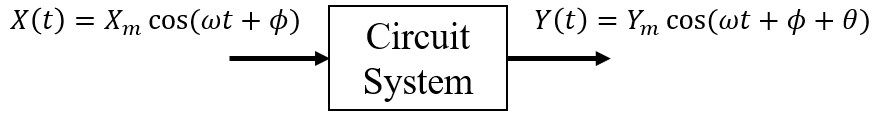
\includegraphics[scale=0.6]{./Linear Circuit System.png}
    \caption{Linear Circuit System}
\end{figure}

각각의 입출력값을 페이저 형식으로 변환하여 표기하면 다음과 같으며 입력 페이저 $\bar{X}$를 바탕으로 페이저 $\bar{Y}$를 출력하는 함수 $H(\omega)$를 정의할 수 있다.

\begin{figure}[h]
    \centering
    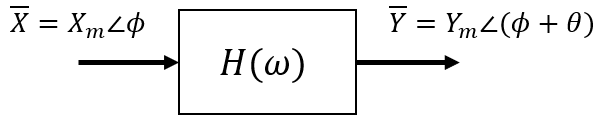
\includegraphics[scale=0.6]{./Frequency Response Function.png}
    \caption{Frequency Response Function}
\end{figure}

이 회로에서 함수 $H(\omega)$를 회로 시스템의 응답 함수라 한다. RLC 회로와 같이 임피던스 $\boldsymbol{Z}=\sqrt{R^2+(X_L-X_C)^2}$를 가지는 회로의 경우 입출력 페이저 간의 진폭과 위상차는 모두 각주파수 $\omega$에 종속적이므로 회로의 응답은 각주파수에 의존한다. 따라서 이 함수 $H(\omega)$가 LTI 선형 회로의 주파수 응답 함수로서 기능하며 다음과 같이 연산할 수 있다.

\begin{equation}
    H(\omega)=\frac{\bar{Y}}{\bar{X}}=\frac{Y_m\angle(\phi+\theta)}{X_m\angle\phi}=\frac{Y_m}{X_m}\angle\theta
\end{equation}

주파수 응답 함수 $H(\omega)$는 회로의 진폭과 위상 변화를 모두 표현하므로 이로부터 진폭 응답과 위상 응답을 유도할 수 있다. 진폭 응답 $A(\omega)$는 주파수에 따른 회로 성분의 진폭 변화를 기술하며 주파수 응답 함수의 실수부를 취하여 다음과 같이 나타낸다.

\begin{equation}
    A(\omega)=\abs{H(\omega)}=\frac{Y_m}{X_m}
\end{equation}

위상 응답 $\phi(\omega)$는 주파수에 따른 회로 성분의 위상 변화를 기술하며 주파수 응답 함수의 허수부를 취하여 나타낸다. 즉, 다음과 같다.

\begin{equation}
    \phi(\omega)=\angle H(\omega)
\end{equation}


\section{대역 필터}
일반적으로 필터는 주파수 영역 중 원하지 않는 성분을 거르거나 원하는 성분만을 추출해 내기 위해 사용되는 회로를 일컫는다. 저항, 축전기, 유도기만을 사용하여 구성된 회로를 수동형 필터회로라 한다. 속도, 온도, 가속도, 힘, 소리 등 다양한 물리량을 계측한 데이터로부터 노이즈를 제거하기 위해 사용되는 필터 회로는 그 특성에 따라 저역통과필터, 고역통과필터, 대역통과필터, 그리고 대역저지필터의 4가지로 구분된다. 대역통과필터(Band-Pass Filter; BPS)는 특정한 주파수를 가진 대역을 통과시키고 그 외의 주파수 대역은 차단하여 노이즈를 제거하는 필터 회로이다. 저항, 유도기, 축전기가 차례로 교류 전원에 연결된 직렬 RLC 회로는 대역 필터의 역할을 수행한다. 다음과 같은 RLC 회로가 있다.

 \begin{figure}[h]
    \centering
    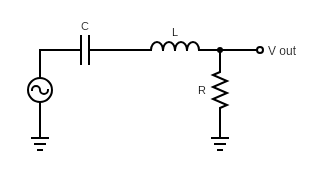
\includegraphics[scale=0.5]{./RLC Circuit.png}
    \caption{RLC Band-Pass Filter}
\end{figure}

이 회로의 전압 성분에 대한 주파수 응답 함수를 구하려면 입력 전압 $V_s$에 대한 출력 전압 $V_o$을 알아야 한다. 전압 분배 법칙에 의하여 $V_o$는 임피던스 $Z$에 대해 다음과 같다.

\begin{equation}
    V_o=\frac{R}{R+Z}
\end{equation}

그런데 $Z=j\omega L+\cfrac{1}{j\omega C}$이므로 식 (16)에 대입하면 다음을 얻는다.

\begin{equation}
    V_o=\frac{R}{R+j(\omega L-\frac{1}{\omega C})}V_s
\end{equation}

식 (13)에 의하여 주파수 응답 함수 $H(\omega)$는 다음과 같다.

\begin{equation}
    H(\omega)=\frac{R}{R+j(\omega L-\frac{1}{\omega C})}
\end{equation}

RLC 회로의 공진은 임피던스가 최소일 때이므로 $Z=j\omega L+\cfrac{1}{j\omega C}$의 허수부가 0일 때 발생한다. 즉, 공진각주파수 $\omega_0=\frac{1}{\sqrt{LC}}$일 때 회로가 공진하고 이때 출력은 최대가 되며 필터링 없이 해당 주파수의 신호를 온전히 수신한다.

\section{시뮬레이션}
Python을 사용하여 직렬 RLC 회로의 주파수 응답 함수 $H(\omega)$를 시각화하였다.

\section{Bibliography}

\end{document}